\pgfplotsset{width=8cm,compat=1.14}
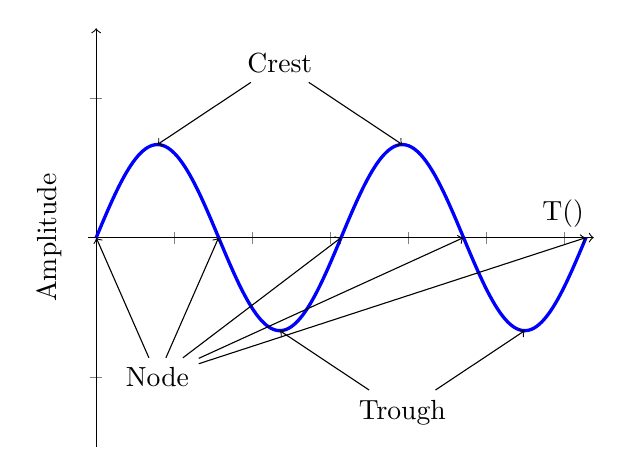
\begin{tikzpicture}
	\begin{axis}
		[
		axis lines=middle,
		axis line style={->},
		xmin=-0.2,
		xmax=4*pi+0.2,
		xticklabels={,,},
		xlabel={T($\si{\second}$)},
		ymin=-1.5,
		ymax=1.5,
		yticklabels={,,},
		ylabel={Amplitude},
		ylabel near ticks,
		]
		\addplot[blue, very thick,samples=200,domain=0:4*pi] {(sin(deg(x)))/1.5};
		\node (crest) at (1.5*pi, 1.25) {Crest};
		\node (trough) at (2.5*pi, -1.25) {Trough};
		\node (node) at (0.5*pi, -1) {Node};
		\draw[->] (crest) -- (0.5*pi, 1/1.5);
		\draw[->] (crest) -- (2.5*pi, 1/1.5);
		\draw[->] (trough) -- (1.5*pi, -1/1.5);
		\draw[->] (trough) -- (3.5*pi, -1/1.5);
		\draw[->] (node) -- (0,0);
		\draw[->] (node) -- (pi,0);
		\draw[->] (node) -- (2*pi,0);
		\draw[->] (node) -- (3*pi,0);
		\draw[->] (node) -- (4*pi,0);
	\end{axis}
\end{tikzpicture}
